\documentclass[a4paper,12pt]{jarticle}
\usepackage[dvipdfmx]{graphicx}
\usepackage{amsmath}
\usepackage{subfigure}
\usepackage{comment}
\usepackage{listings}

\setlength{\hoffset}{0cm}
\setlength{\oddsidemargin}{-3mm}
\setlength{\evensidemargin}{-3cm}
\setlength{\marginparsep}{0cm}
\setlength{\marginparwidth}{0cm}
\setlength{\textheight}{24.7cm}
\setlength{\textwidth}{17cm}
\setlength{\topmargin}{-45pt}

\renewcommand{\baselinestretch}{1.6}
\renewcommand{\floatpagefraction}{1}
\renewcommand{\topfraction}{1}
\renewcommand{\bottomfraction}{1}
\renewcommand{\textfraction}{0}
\renewcommand{\labelenumi}{(\arabic{enumi})}
%\renewcommand{\figurename}{Fig.} %図をFig.にする


%図のキャプションからコロン:を消す
\makeatletter
\long\def\@makecaption#1#2{% #1=図表番号、#2=キャプション本文
\sbox\@tempboxa{#1. #2}
\ifdim \wd\@tempboxa >\hsize
#1 #2\par 
\else
\hb@xt@\hsize{\hfil\box\@tempboxa\hfil}
\fi}
\makeatother
% 

%Listingnameの定義
\def\lstlistingname{Program}
%
\title{車両制御特論 \\
レポート1\\
}
\author{\vspace{40mm}\\
九州工業大学大学院 \hspace{0mm} 工学府\\
機械知能工学専攻\ \hspace{0mm} 知能制御工学コース \\
\vspace{5mm}\\
所属:\ 西田研究室\\
学籍番号:\ 16344217\\
提出者氏名:\ 津上 \hspace{0mm} 祐典\\\vspace{5mm}\\ }
\date{平成28年\ 7月\ 19日}

\begin{document}

%表紙
\titlepage
\maketitle
\thispagestyle{empty}

\newpage
%%%%%%%%%%%%%%%%%%%%%%%%%%%%
\section{与えられたシステム}
%%%%%%%%%%%%%%%%%%%%%%%%%%%
学籍番号より決定した解析するシステムは
\begin{eqnarray}\label{equ:sys}
 \begin{cases}
  \dot{x}(t) = -4x(t) + 6u_{4}(t) \ , \  x(0) = -5 \\
  u_{4}(t) = -2-\sin t &
 \end{cases}
\end{eqnarray}
である.
%
%%%%%%%%%%%%%%%%%%%%%%%%%%%
\section{システムの解析解}
%%%%%%%%%%%%%%%%%%%%%%%%%%%
(\ref{equ:sys})式で示したシステムの解析解$x(t)$を導出する.
(\ref{equ:sys})式より
%
\begin{eqnarray}
 \dot{x}(t) &=& -4x(t) + 6(-2-\sin t) \\
 \dot{x}(t) &=& -4x(t) -12 -6\sin t
\end{eqnarray}
%
となる.上式の両辺をラプラス変換し,整理すると,
%
\begin{eqnarray}
 sX(s) + 5 & = & -4X(s) - \frac{12}{s} - \frac{6}{s^2 + 1} \\
 (s+5)X(s) & = & -5 - \frac{12}{s} - \frac{6}{s^2 + 1} \\
 X(s) & = & -\frac{5}{s+4} - \frac{12}{s(s+4)} - \frac{6}{(s^2 + 1)(s+4)} \\
 X(s) & = & -\frac{5}{s+4} - 12 (\frac{\frac{1}{4}}{s} -
  \frac{\frac{1}{4}}{s+4}) -6(\frac{-\frac{1}{17}s+\frac{4}{17}}{s^2 +
  1}+\frac{\frac{1}{17}}{s+4}) \\
 X(s) & = & -\frac{40}{17}\frac{1}{s+4} + \frac{6}{17}\frac{s}{s^2 + 1}
  -\frac{24}{17}\frac{1}{s^2 + 1} -\frac{3}{s}
 \end{eqnarray}
となる.ただし,$X(s)$は$x(t)$をラプラス変換したものである.そして,上式
の両辺を逆ラプラス変換すればシステムの解析解
%
\begin{equation}
 x(t)  =  -\frac{40}{17}e^{-4t} + \frac{6}{17}\cos t -\frac{24}{17}\sin t -3
\end{equation}
%
を得る.
%%%%%%%%%%%%%%%%%%%%%%%%%%%%%%%%%%%%%%%%%%
\section{Simulink,MATLABのプログラム}
%%%%%%%%%%%%%%%%%%%%%%%%%%%%%%%%%%%%%%%%%%
(\ref{equ:sys})式で示されるシステムをSimulinkのモデルを図\ref{fig:model}に,MATLABのプログラ
ムをProgram 1.に示す.
%
\begin{figure}[hbp]
 \begin{center}
  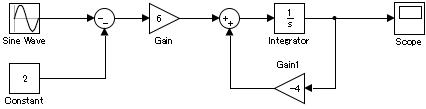
\includegraphics[scale=.7,bb = 0 0 426 109]{fig/model.jpg}
 \end{center}
 \caption{作成したsimulinkモデル}
 \label{fig:model}
\end{figure}
%
\begin{lstlisting}[basicstyle=\ttfamily\footnotesize,frame=single,caption=作成したMATLABのプログラム]
clc;
clear;
clf;
sim('model');
figure(1);
x_a = -(40/17)*exp(-4*t.time)+(6/17)*cos(t.time)-(24/17)*sin(t.time)-3; 
plot(t.time,x_a,'-',t.time,y.signals.values,'-');
legend('Analytic value','Simulation value');
xlabel('time [s]');
ylabel('x(t)')

figure(2);
plot(t.time,y.signals.values,'-');
legend('Simulation value');
xlabel('time [s]');
ylabel('x(t)')

figure(3);
x_a = -(40/17)*exp(-4*t.time)+(6/17)*cos(t.time)-(24/17)*sin(t.time)-3; 
plot(t.time,x_a,'-');
legend('Analytic value');
xlabel('time [s]');
ylabel('x(t)')
\end{lstlisting}

%%%%%%%%%%%%%%%%%%%%%%%%%
\section{得られた応答}
%%%%%%%%%%%%%%%%%%%%%%%%
%
得られた応答波形を図\ref{fig:output}にそれぞれ示す.また,解析解をプロッ
トしたもの,シミュレーション結果を同時にプロット
したものを図\ref{fig:text2}に示す.
%
\begin{figure}[htbp]
  \begin{center} 
   \subfigure[解析解をプロットしたもの]{
   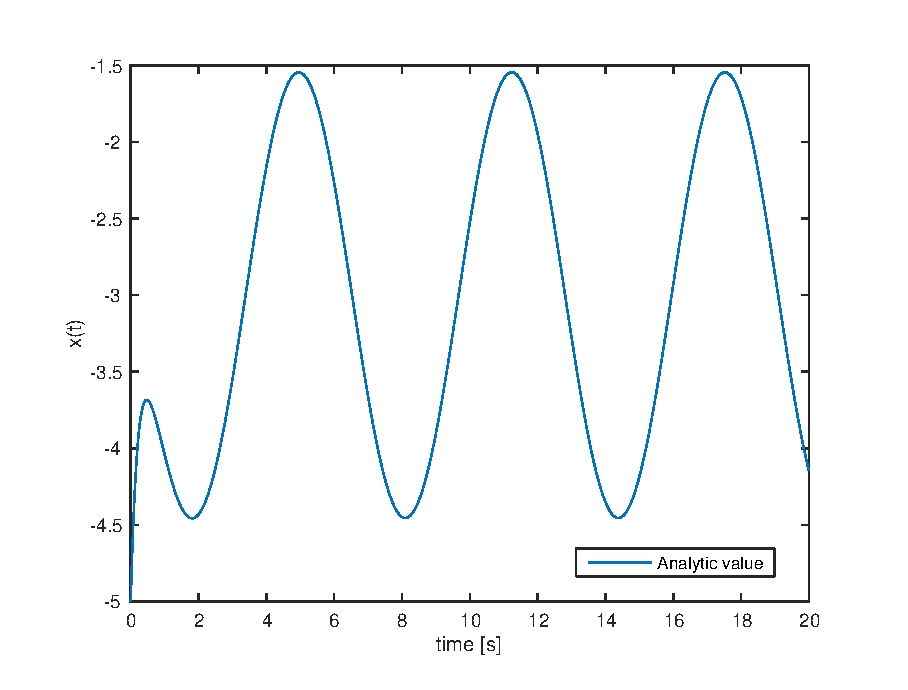
\includegraphics[scale=.55]{fig/analy.eps}  
     \label{fig:kaiseki}
  }
  %
  \hfill
  %
  \subfigure[Matlab/Simulinkでシミュレーションした結果]{
   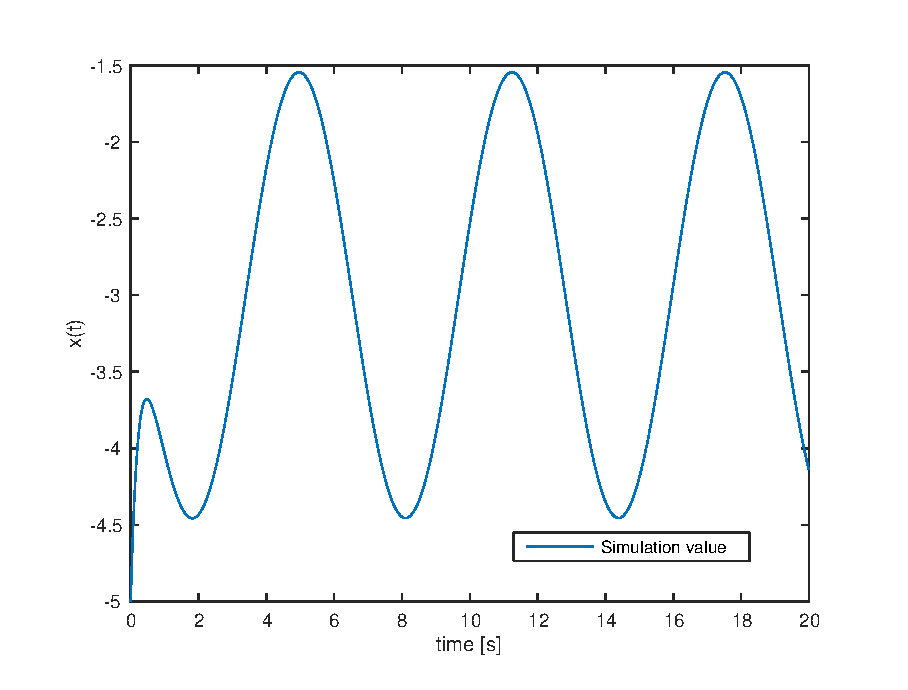
\includegraphics[scale=.55]{fig/simu.eps}
   \label{fig:simu}
  }
  \end{center}
  \caption{得られた応答}
  \label{fig:output}
\end{figure}
%
\begin{figure}[bp]
 \begin{center}
  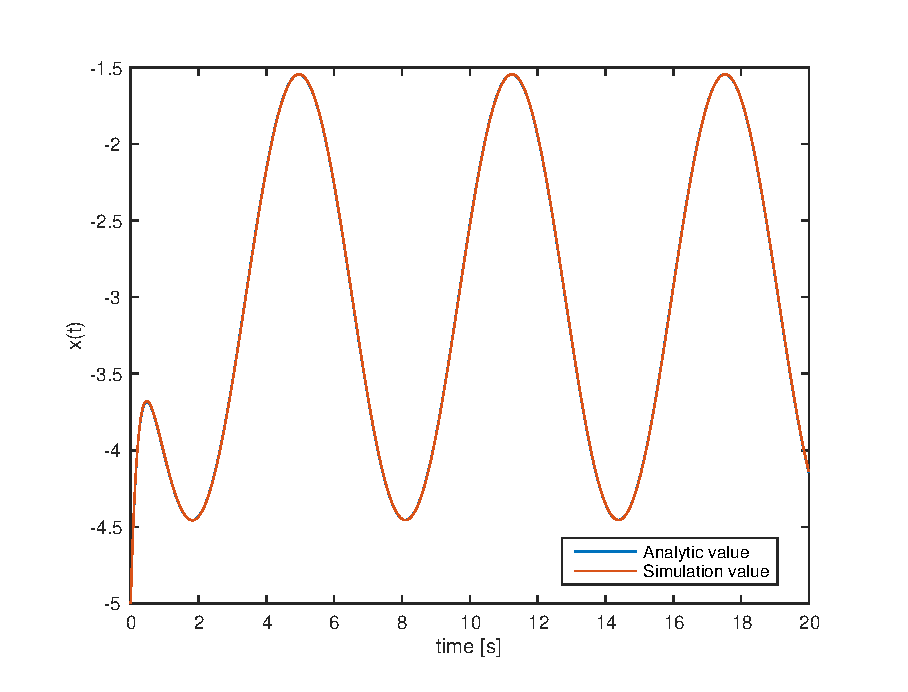
\includegraphics[scale=.9]{fig/multi.eps}
 \end{center}
 \caption{Matlab/Simulinkによるシミュレーション結果と解析解のプロットとの比較}
 \label{fig:text2}
\end{figure}
%
%%%%%%%%%%%%%%%%%%%%%%%%
\section{考察}
%%%%%%%%%%%%%%%%%%%%%%%%
図\ref{fig:text2}を見ると,二つの波形いずれも定常応答において$x(t)=-3$を中心
として振動していることがわかる.また,二つの波形が一致していることを確認
した.今回は,システムが簡単であったため解析解を求め,プロットすることが
できるが,システムが複雑であると解析解を求めることが困難であると考えられ
る.
%
%
\begin{thebibliography}{99}
\addcontentsline{toc}{section}{参考文献}

 \bibitem{jamming} 大屋勝敬:"車両制御特論MATLAB+Simulinkの利用法"
\end{thebibliography}

\end{document}
